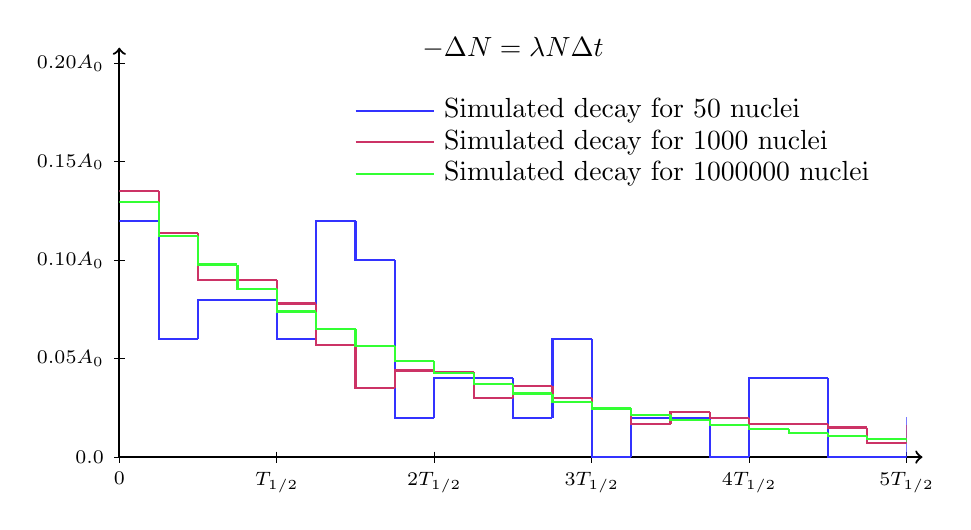
\begin{tikzpicture}
\node[] at (5.0,5.2) {$-\Delta N = \lambda N \Delta t$};
\draw[thick,->] (0.0,0.0) -- (0.0,5.2);
\draw[thick,->] (0.0,0.0) -- (10.2,0.0);
\draw (0,0cm + 2pt) -- (0, 0cm-2pt) node[below] {\scriptsize $0$};
\draw (2,0cm + 2pt) -- (2, 0cm-2pt) node[below] {\scriptsize $T_{1/2}$};
\draw (4,0cm + 2pt) -- (4, 0cm-2pt) node[below] {\scriptsize $2T_{1/2}$};
\draw (6,0cm + 2pt) -- (6, 0cm-2pt) node[below] {\scriptsize $3T_{1/2}$};
\draw (8,0cm + 2pt) -- (8, 0cm-2pt) node[below] {\scriptsize $4T_{1/2}$};
\draw (10,0cm + 2pt) -- (10, 0cm-2pt) node[below] {\scriptsize $5T_{1/2}$};
\draw (0cm+2pt,0.    ) -- (0cm-2pt,0.    ) node[left] {\scriptsize $0.0$};
\draw (0cm+2pt,1.25    ) -- (0cm-2pt,1.25    ) node[left] {\scriptsize $0.05 A_0$};
\draw (0cm+2pt,2.5    ) -- (0cm-2pt,2.5    ) node[left] {\scriptsize $0.10 A_0$};
\draw (0cm+2pt,3.750000093132256    ) -- (0cm-2pt,3.750000093132256    ) node[left] {\scriptsize $0.15 A_0$};
\draw (0cm+2pt,5.    ) -- (0cm-2pt,5.    ) node[left] {\scriptsize $0.20 A_0$};
\begin{scope}[]
\clip (0,0) rectangle (10,5);
\draw[blue!80,thick] (3.0,4.4) -- (4.0,4.4);
\node[right,] at (4.0,4.4) {Simulated decay for 50 nuclei};
\begin{scope}[blue!80,thick]
\draw[] (0.0,2.999999955296517) -- (0.5,2.999999955296517);
\draw (0.5,2.999999955296517) -- (0.5,1.4999999776482584) -- (1.0,1.4999999776482584);
\draw (1.0,1.4999999776482584) -- (1.0,1.999999970197678) -- (1.5,1.999999970197678);
\draw (1.5,1.999999970197678) -- (1.5,1.999999970197678) -- (2.0,1.999999970197678);
\draw (2.0,1.999999970197678) -- (2.0,1.4999999776482584) -- (2.5,1.4999999776482584);
\draw (2.5,1.4999999776482584) -- (2.5,2.999999955296517) -- (3.0,2.999999955296517);
\draw (3.0,2.999999955296517) -- (3.0,2.4999999627470975) -- (3.5,2.4999999627470975);
\draw (3.5,2.4999999627470975) -- (3.5,0.4999999925494195) -- (4.0,0.4999999925494195);
\draw (4.0,0.4999999925494195) -- (4.0,0.999999985098839) -- (4.5,0.999999985098839);
\draw (4.5,0.999999985098839) -- (4.5,0.999999985098839) -- (5.0,0.999999985098839);
\draw (5.0,0.999999985098839) -- (5.0,0.4999999925494195) -- (5.5,0.4999999925494195);
\draw (5.5,0.4999999925494195) -- (5.5,1.4999999776482584) -- (6.0,1.4999999776482584);
\draw (6.0,1.4999999776482584) -- (6.0,0.0) -- (6.5,0.0);
\draw (6.5,0.0) -- (6.5,0.4999999925494195) -- (7.0,0.4999999925494195);
\draw (7.0,0.4999999925494195) -- (7.0,0.4999999925494195) -- (7.5,0.4999999925494195);
\draw (7.5,0.4999999925494195) -- (7.5,0.0) -- (8.0,0.0);
\draw (8.0,0.0) -- (8.0,0.999999985098839) -- (8.5,0.999999985098839);
\draw (8.5,0.999999985098839) -- (8.5,0.999999985098839) -- (9.0,0.999999985098839);
\draw (9.0,0.999999985098839) -- (9.0,0.0) -- (9.5,0.0);
\draw (9.5,0.0) -- (9.5,0.0) -- (10.0,0.0);
\draw (10.0,0.0) -- (10.0,0.4999999925494195) -- (10.5,0.4999999925494195);
\draw (10.5,0.4999999925494195) -- (10.5,0.999999985098839) -- (11.0,0.999999985098839);
\draw (11.0,0.999999985098839) -- (11.0,0.0) -- (11.5,0.0);
\draw (11.5,0.0) -- (11.5,0.0) -- (12.0,0.0);
\draw (12.0,0.0) -- (12.0,0.0) -- (12.5,0.0);
\end{scope}
\draw[purple!80,thick] (3.0,4.0) -- (4.0,4.0);
\node[right,] at (4.0,4.0) {Simulated decay for 1000 nuclei};
\begin{scope}[purple!80,thick]
\draw[] (0.0,3.374999949708582) -- (0.5,3.374999949708582);
\draw (0.5,3.374999949708582) -- (0.5,2.849999957531691) -- (1.0,2.849999957531691);
\draw (1.0,2.849999957531691) -- (1.0,2.2499999664723878) -- (1.5,2.2499999664723878);
\draw (1.5,2.2499999664723878) -- (1.5,2.2499999664723878) -- (2.0,2.2499999664723878);
\draw (2.0,2.2499999664723878) -- (2.0,1.949999970942736) -- (2.5,1.949999970942736);
\draw (2.5,1.949999970942736) -- (2.5,1.4249999787658456) -- (3.0,1.4249999787658456);
\draw (3.0,1.4249999787658456) -- (3.0,0.8749999869614842) -- (3.5,0.8749999869614842);
\draw (3.5,0.8749999869614842) -- (3.5,1.0999999836087229) -- (4.0,1.0999999836087229);
\draw (4.0,1.0999999836087229) -- (4.0,1.0749999839812518) -- (4.5,1.0749999839812518);
\draw (4.5,1.0749999839812518) -- (4.5,0.7499999888241292) -- (5.0,0.7499999888241292);
\draw (5.0,0.7499999888241292) -- (5.0,0.8999999865889551) -- (5.5,0.8999999865889551);
\draw (5.5,0.8999999865889551) -- (5.5,0.7499999888241292) -- (6.0,0.7499999888241292);
\draw (6.0,0.7499999888241292) -- (6.0,0.6249999906867744) -- (6.5,0.6249999906867744);
\draw (6.5,0.6249999906867744) -- (6.5,0.4249999936670066) -- (7.0,0.4249999936670066);
\draw (7.0,0.4249999936670066) -- (7.0,0.5749999914318324) -- (7.5,0.5749999914318324);
\draw (7.5,0.5749999914318324) -- (7.5,0.4999999925494195) -- (8.0,0.4999999925494195);
\draw (8.0,0.4999999925494195) -- (8.0,0.4249999936670066) -- (8.5,0.4249999936670066);
\draw (8.5,0.4249999936670066) -- (8.5,0.4249999936670066) -- (9.0,0.4249999936670066);
\draw (9.0,0.4249999936670066) -- (9.0,0.3749999944120646) -- (9.5,0.3749999944120646);
\draw (9.5,0.3749999944120646) -- (9.5,0.17499999739229682) -- (10.0,0.17499999739229682);
\draw (10.0,0.17499999739229682) -- (10.0,0.3999999940395356) -- (10.5,0.3999999940395356);
\draw (10.5,0.3999999940395356) -- (10.5,0.12499999813735488) -- (11.0,0.12499999813735488);
\draw (11.0,0.12499999813735488) -- (11.0,0.12499999813735488) -- (11.5,0.12499999813735488);
\draw (11.5,0.12499999813735488) -- (11.5,0.12499999813735488) -- (12.0,0.12499999813735488);
\draw (12.0,0.12499999813735488) -- (12.0,0.14999999776482587) -- (12.5,0.14999999776482587);
\end{scope}
\draw[green!80,thick] (3.0,3.6) -- (4.0,3.6);
\node[right,] at (4.0,3.6) {Simulated decay for 1000000 nuclei};
\begin{scope}[green!80,thick]
\draw[] (0.0,3.234924951795862) -- (0.5,3.234924951795862);
\draw (0.5,3.234924951795862) -- (0.5,2.8036749582219875) -- (1.0,2.8036749582219875);
\draw (1.0,2.8036749582219875) -- (1.0,2.445724963555858) -- (1.5,2.445724963555858);
\draw (1.5,2.445724963555858) -- (1.5,2.137424968149886) -- (2.0,2.137424968149886);
\draw (2.0,2.137424968149886) -- (2.0,1.8491249724458907) -- (2.5,1.8491249724458907);
\draw (2.5,1.8491249724458907) -- (2.5,1.6278999757423998) -- (3.0,1.6278999757423998);
\draw (3.0,1.6278999757423998) -- (3.0,1.4105749789807949) -- (3.5,1.4105749789807949);
\draw (3.5,1.4105749789807949) -- (3.5,1.2250749817449602) -- (4.0,1.2250749817449602);
\draw (4.0,1.2250749817449602) -- (4.0,1.0674999840930106) -- (4.5,1.0674999840930106);
\draw (4.5,1.0674999840930106) -- (4.5,0.9282749861676247) -- (5.0,0.9282749861676247);
\draw (5.0,0.9282749861676247) -- (5.0,0.8072749879706652) -- (5.5,0.8072749879706652);
\draw (5.5,0.8072749879706652) -- (5.5,0.7039999895095826) -- (6.0,0.7039999895095826);
\draw (6.0,0.7039999895095826) -- (6.0,0.6185249907832594) -- (6.5,0.6185249907832594);
\draw (6.5,0.6185249907832594) -- (6.5,0.5318249920751901) -- (7.0,0.5318249920751901);
\draw (7.0,0.5318249920751901) -- (7.0,0.46762499303184457) -- (7.5,0.46762499303184457);
\draw (7.5,0.46762499303184457) -- (7.5,0.4117999938637019) -- (8.0,0.4117999938637019);
\draw (8.0,0.4117999938637019) -- (8.0,0.35572499469928454) -- (8.5,0.35572499469928454);
\draw (8.5,0.35572499469928454) -- (8.5,0.3076749954152853) -- (9.0,0.3076749954152853);
\draw (9.0,0.3076749954152853) -- (9.0,0.26714999601915485) -- (9.5,0.26714999601915485);
\draw (9.5,0.26714999601915485) -- (9.5,0.23472499650232498) -- (10.0,0.23472499650232498);
\draw (10.0,0.23472499650232498) -- (10.0,0.2072499969117344) -- (10.5,0.2072499969117344);
\draw (10.5,0.2072499969117344) -- (10.5,0.1727749974254519) -- (11.0,0.1727749974254519);
\draw (11.0,0.1727749974254519) -- (11.0,0.15319999771714213) -- (11.5,0.15319999771714213);
\draw (11.5,0.15319999771714213) -- (11.5,0.13352499801032247) -- (12.0,0.13352499801032247);
\draw (12.0,0.13352499801032247) -- (12.0,0.11539999828040602) -- (12.5,0.11539999828040602);
\end{scope}
\end{scope}
\end{tikzpicture}
%%% Local Variables: 
%%% mode: latex 
%%% TeX-master: "master" 
%%% End:

